\begin{figure}[t]

\begin{minipage}[b]{0.50\linewidth}
{
    \centering 
    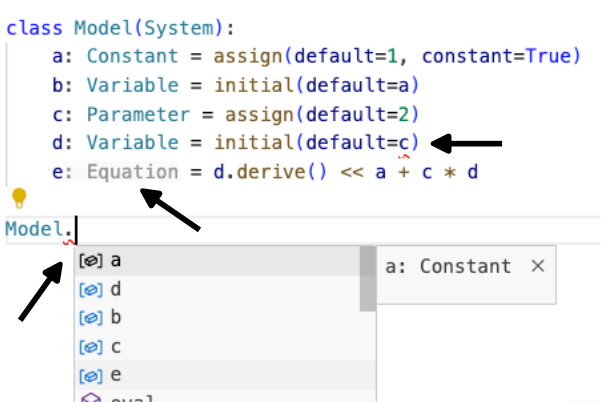
\includegraphics{src/ide/ide1.pdf}
}
\end{minipage}%
%
\begin{minipage}[b]{0.50\linewidth}
{
    \centering
    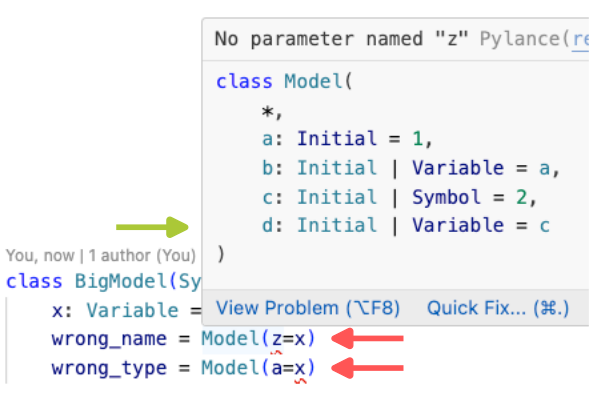
\includegraphics{src/ide/ide2.pdf}
}
\end{minipage}%

\caption{
    \label{fig-ide}
    Screenshots of Visual Studio Code showing
    tooltips (green arrows) and
    highlighted type errors (red arrows).
    On the left,
    we show that \texttt{a},
    a \texttt{Constant} assigned with \texttt{assign(...,\ constant=True)},
    can be used for \texttt{Variable b}'s initial condition.
    Instead,
    it is flagged as a type error (red underlining)
    when using \texttt{c}, a \texttt{Parameter},
    for \texttt{Variable d}'s initial condition,
    The IDE automatically recognizes \texttt{e} as an \texttt{Equation},
    and provides autocompletion of the \texttt{Model}'s components.
    A tooltip is shown when composing models (green arrow, right),
    which show the expected variables and their default values.
    The IDE highlights wrong names (\texttt{z} is not a name in \texttt{Model})
    and mismatched types (\texttt{x} is \texttt{Variable} and \texttt{a} must be a number or a \texttt{Constant})
}

\end{figure}
